\documentclass[a4paper, 12pt, twoside]{article}
\usepackage[outer={2.5cm},inner={4cm},tmargin={2.5cm},bmargin={2cm}]{geometry}
\usepackage{amsmath}
\usepackage{amssymb}
\usepackage{amsthm}
\usepackage{babel}[english]
\usepackage{hyperref}
\usepackage{colonequals}
\usepackage{xfrac}
\usepackage{tikz}
\usepackage{tikz-cd}
\usepackage{stmaryrd}
\usepackage{enumitem}
\usepackage{faktor}
\usepackage{enumitem}
\usepackage{dsfont}
\usepackage[style=numeric,backend=biber]{biblatex}

\usepackage{graphicx}
\usepackage{caption}

\setlength{\parindent}{0mm}
\setcounter{MaxMatrixCols}{100}

\newcommand{\N}[0]{\mathbb{N}}
\newcommand{\Z}[0]{\mathbb{Z}}
\newcommand{\R}[0]{\mathbb{R}}
\newcommand{\NB}[0]{\mathcal{N}}
\newcommand{\T}[0]{\mathcal{T}}
\newcommand{\F}[0]{\mathcal{F}}
\newcommand{\PowS}[0]{\mathfrak{P}}
\newcommand{\PowSF}[0]{\mathfrak{P}_{\text{fin}}}
\newcommand*{\logeq}{\ratio\Leftrightarrow}
\newcommand*{\longeq}{\ratio\Longleftrightarrow}
\newcommand*{\bigdot}{\mathpalette\bigcdot@{.5}}
\newcommand{\sd}{{\rm sd}}
\newcommand{\dom}{{\rm dom}}
\newcommand{\cone}{{\rm Cone}}
\newcommand{\id}{{\rm id}}
\newcommand{\im}{{\rm im}}
\newcommand{\Q}{\mathcal{Q}}
\renewcommand{\P}{\mathcal{P}}
\newcommand*{\anddot}{%
  \mathclose{}%
  \nonscript\mskip.5\thinmuskip
  \boldsymbol{.}%
  \;%
  \mathopen{}%
}
\newcommand\restr[2]{{% we make the whole thing an ordinary symbol
  \left.\kern-\nulldelimiterspace % automatically resize the bar with \right
  #1 % the function
  \littletaller % pretend it's a little taller at normal size
  \right|_{#2} % this is the delimiter
  }}

\newcommand{\littletaller}{\mathchoice{\vphantom{\big|}}{}{}{}}

\usepackage{colonequals}
%\newcommand*{\logeq}{\ratio\Leftrightarrow}
%\newcommand*{\longeq}{\ratio\Longleftrightarrow}
  
\title{Master Thesis\\{$L^0$-groups, extreme amenability, and algebraic topology}}
\author{Yannik Höll}
\date{\today}

\newtheoremstyle{break}%
{7pt}{7pt}%
{}{}%
{\bfseries}{:}% % Note that final punctuation is omitted.
{\newline}{}

\theoremstyle{break}
\newtheorem{thm}{Theorem}[section]

\theoremstyle{break}
\newtheorem{rem}[thm]{Remark}
\newtheorem{lemma}[thm]{Lemma}
\newtheorem{defin/}[thm]{Definition}
\newtheorem{col}[thm]{Corollary}
\newtheorem{ex}[thm]{Example}
\newtheorem{cons}[thm]{Construction}

\newenvironment{defin}
    {\renewcommand{\qedsymbol}{$\spadesuit$}\pushQED{\qed}\begin{defin/}}
    {\popQED\end{defin/}}

% for centering the title page
\usepackage{titling}

\usepackage{nomencl}
\makenomenclature

\nomenclature{$\chi(G)$}{The chromatic number of the graph $G$, i.e., the smallest number of colors needed for a proper vertex coloring}
\nomenclature{$\mathcal{T}_X$}{The topology of the top. space $X$}
\nomenclature{$\mathbb{S}^n$}{The $n$-dimensional sphere for $n \in \N$.}
\nomenclature{$B_\varepsilon(x)$}{The open ball with radius $\varepsilon \in \R_{>0}$ in a metric space $X$ around $x \in X$}
\nomenclature{$d_X$}{The metric of the metric space $X$}
\nomenclature{$X^Y$}{The set of all maps from $Y$ to $X$}
\nomenclature{$C(X, Y)$}{The set of all continuous functions between top. spaces $X$ and $Y$}
\nomenclature{$\{\rm Flt}(X)$}{The set of all filters on a set $X$}
\nomenclature{$\{\rm UFlt}(X)$}{The set of all ultrafilters on a set $X$}
\nomenclature{$\mid \hspace*{-2px} X \hspace*{-2px}\mid$}{The cardinality of the set $X$}
\nomenclature{$[n]$}{The set $\{0, 1, \ldots, n-1\}$ for a natural number $n$}
\nomenclature{$[k,n]$}{The set $[n]\setminus[k]$ for natural numbers $n \geq k$}
\nomenclature{$X^c$}{The complement of the set $X$}
\nomenclature{$\PowS(X)$}{The set of all subsets of $X$}
\nomenclature{$\PowS_{\leq n}(X)$}{The set of all subsets of $X$ with cardinality less than or equal to $n \in \N$}
\nomenclature{$\PowSF(X)$}{The set of all finite subsets of $X$}
\nomenclature{$\dom(f)$}{The domain of the map $f$ or relation $f$}
\nomenclature{$\im(f)$}{The image of the map $f$ or relation $f$}
\nomenclature{$\id_X$}{The map $X \to X, \: x \mapsto x$ on a set $X$}
\nomenclature{$\mathds{1}_x$}{The indicator map for $x \in X$ on a set $X$}
\nomenclature{$\N^+$}{The set of natural numbers excluding 0}
\nomenclature{$\N$}{The set of natural numbers including 0}
\nomenclature{$\mathcal{N}_X(x)$}{The set of all open sets in a top. space $X$ containing the element $x \in X$}
\nomenclature{$\mathbb{P}$}{The set of prime numbers}
\nomenclature{$\R$}{The set of real numbers}
\nomenclature{$\R_{> 0}$}{The set of real numbers greater than 0}
\nomenclature{$\Z$}{The set of integers}
\nomenclature{$\Z_p$}{The group of integers modulo a prime $p$ with addition modulo $p$}
\nomenclature{$\underline{\rm Top}$}{The category of topological spaces with continuous functions as arrows}
\nomenclature{$\underline{\rm Ab}$}{The category of abelian groups with group homomorphisms as arrows}
\nomenclature{$\underline{\rm Grp}$}{The category of groups with group homomorphisms as arrows}
\nomenclature{$\underline{\rm Ab}(G, H)$}{The class of all homomorphisms between the two abelian groups $G$ and $H$}
\nomenclature{$\underline{\rm Grp}(G, H)$}{The class of all homomorphisms between the two groups $G$ and $H$}
\nomenclature{$P(X,Y)$}{Set of non-empty partial functions from $X$ to $Y$}
\nomenclature{$X \sqcup Y$}{Disjoint union of the sets $X$ and $Y$, defined as, $X \sqcup Y = (X \times \{0\}) \cup (Y \times \{1\})$}
\usepackage{setspace} % Allows control over line spacing
\renewcommand{\nompreamble}{\begin{flushleft} \setstretch{0.9}} % Align left & reduce line spacing
\renewcommand{\nompostamble}{\end{flushleft}}  % End alignment
\renewcommand{\nomlabelwidth}{10em} % Space allocated for symbols
\renewcommand{\nomlabel}[1]{\hspace{0pt}#1\dotfill} % Dots between symbol and description
\setlength{\nomitemsep}{-0.8em} % Adjust spacing between entries

\renewcommand{\nomname}{List of Symbols} % Change title

\renewbibmacro{in:}{%
  \ifentrytype{article}{\printtext{\bibstring{in}\addnbspace}}{}%
}


\usepackage{tocloft}

% Reduce vertical spacing in TOC
\setlength{\cftbeforesecskip}{0pt} % No space before section entries
\setlength{\cftbeforesubsecskip}{0pt} % No space before subsection entries
\setlength{\cftbeforesubsubsecskip}{0pt} % No space before subsubsection entries


\addbibresource{references.bib}
\linespread{1.5}
\begin{document}

\begin{titlingpage}
    \maketitle
\end{titlingpage}
\clearpage

\vspace*{\fill}
\begin{center}
\textit{
    I would like to thank all proofreaders that have helped me correcting the errors in this thesis. 
    And special thanks to Prof. Schneider who has answered many of my questions concerning the material discussed in this thesis.  
}
\end{center}
\vspace*{\fill}
\thispagestyle{empty}
\clearpage

\tableofcontents
\vspace*{11cm}
\pagebreak

\printnomenclature
\pagebreak

\nocite{*}

\section{Introduction}

The main results from Sections \ref{sec:l0groups}, \ref{sec:borsuk} and \ref{sec:bounds} originated in the work of Marcin Sabok \cite{sabok2012}. 

\section{Topology, Topological Algebra and Algebraic Topology}
In this whole section, $X$ will be a set.

\subsection{Topology}

\begin{defin}
  A \textbf{topology} $\mathcal{T}$ on $X$ is a collection of subsets of $X$ obeying the follwing axioms
  \begin{enumerate}
    \item $X \in \mathcal{T} \ni \emptyset$,
    \item $\bigcup\limits_{\alpha \in I}A_{\alpha} \in \mathcal{T}$, where $I$ is an abitrary index set and $A_{\alpha} \in \mathcal{T}$ for all $\alpha \in I$,
    \item $\bigcap\limits_{i=0}^n A_i$ for $n \in \N$ and $A_i \in \mathcal{T}$.
  \end{enumerate}
\end{defin}

\begin{defin}
  A \textbf{filter} $\mathcal{F}$ on a set $X$ is a collection of subsets of $X$ such that:
  \begin{enumerate}
    \item $X \in \mathcal{F}$, $\emptyset \notin \mathcal{F}$,
    \item $\forall A, B \in \mathcal{F}\colon A\cap B \in \mathcal{F}$,
    \item $\forall A \subseteq B \subseteq X: A \in \mathcal{F} \Rightarrow B \in \mathcal{F}$.
  \end{enumerate}
\end{defin}

\begin{defin} 
  An \textbf{ultrafilter} $\mathcal{F}$ on $X$ is a filter on $X$ with the property that if there is another filter on X called $\mathcal{F}'$ such that $\mathcal{F} \subseteq \mathcal{F}'$ it follows that $\mathcal{F} = \mathcal{F}'$.
  If $\bigcap \mathcal{F} = \emptyset$ the ultrafilter is called \textbf{non-principle}.
\end{defin}

\subsection{Topological Algebra}

\subsection{Algebraic Topology}

\section{Simplicial Homology}

\subsection{Abstract simplicial complexes}

\begin{defin}
    Let $X$ be a non-empty set. Then a collection $\mathcal{K} \subseteq \PowS(X)$ of subsets of $X$ is called a 
    \textbf{simplicial complex} on $X$ if
    \begin{equation*}
        \forall G\in\mathcal{K} \colon F \subseteq G \; \Rightarrow \; F \in \mathcal{K}.
    \end{equation*}
    The elements of the set $V(\mathcal{K}) := \bigcup \mathcal{K}$ are the \textbf{vertecies} of $\mathcal{K}$ and
    elements of $\mathcal{K}$ itself are the \textbf{simplicies}. Given a simplex $\sigma \in \mathcal{K}$ then the sets
    $\; \sigma \setminus \{x\} \;$ for $x \in \sigma$ are called the \textbf{faces} of $\sigma$.
    Let $Y$ be another non-empty set and $\mathcal{L}$ be a simplicial complex on $Y$. A map $f: V(\mathcal{K}) \to V(\mathcal{L})$ is called 
    a \textbf{simplicial} map if
    \begin{equation*}
        \forall \sigma \in \mathcal{K}\colon f(\sigma) \in \mathcal{L}.
    \end{equation*}
    If $f$ is bijective it is an \textbf{combinatorial isomorphism}.
\end{defin}

% Simple example of a simplicial complex

\begin{defin}
    Let $X$ be a set, $H$ be a group and $\mathcal{K}$ be a simplicial complex on $X$. If there is an 
    group action $\lambda \colon H \times X \to X$ of $H$ on $X$ then
    the complex $\mathcal{K}$ is an \textbf{$H$-complex} if the map
    \begin{equation*}
        \lambda_h \colon \mathcal{K} \to \mathcal{K}, \: \sigma \mapsto \{ \lambda(h, \tau)\colon \tau \in \sigma \}
    \end{equation*}
    is a simplicial map for all $h \in H$.
\end{defin}

\begin{defin}
    A poset (partially ordered set) is a pair $(P, \preceq)$ where 
    $P$ is a non-empty set and 
    $\preceq$ is a binary relation on $P$ which has the following properties:
    \begin{enumerate}
        \item \textit{Reflexivity}: $\forall x \in P\colon x \preceq x$,
        \item \textit{Antisymmetry}: $\forall x, y \in P\colon (x \preceq y \: \land \: y \preceq x) \Rightarrow (x = y)$,
        \item \textit{Transitivity}: $\forall x, y, z \in P\colon (x \preceq y \: \land \: y \preceq z) \Rightarrow (x \preceq z)$.
    \end{enumerate}
    A chain in $P$ is a subset $C \subseteq P$ which is totally ordered, i.e.
    \begin{equation*}
        \forall x, y \in C\colon x \preceq y \: \lor \: y \preceq x.
    \end{equation*}
\end{defin}

\begin{ex}
    If $X$ is a non-empty set then the pair $(\PowS(X), \subseteq)$ forms a poset.
\end{ex}

The last example establishes the following definition:
If $X$ is a non-empty family of sets then $P(X) := (X, \subseteq)$ is the poset generated by $X$. The elements of $X$
are the elements of the poset and the binary relation of set inclusion is the partial order.

\begin{defin}
    Let $\mathcal{K}$ be an abstract simplicial complex. The \textbf{barycentric subdivision} $\sd(\mathcal{K})$ of $\mathcal{K}$
    is the abstract simplicial complex with $\mathcal{K}$ as the set of vertecies and all chains in $P(\mathcal{K})$ as simplicies.
\end{defin}

\begin{thm}
    If $\mathcal{K}$ is a abstract simplicial complex, then $\sd(\mathcal{K})$ is a well-defined abstract simplicial complex.
\end{thm}

\begin{proof}
    Let $\sigma \in \sd(\mathcal{K})$. Now let $\tau \subseteq \sigma$. Since $\sigma$ was totally ordered $\tau$ is also totally ordered.
    This means that $\tau \in \mathcal{K}$.
\end{proof}

% TODO: example of barycentric subdivision of the triangle simplex 1,2,3

\subsection{Geometric simplicial complexes}

In the following, we will discuss another class of simplicial complexes. 
This time, they will be subspaces of the $n$-dimensional euclidian space.
These complexes will be polyhedra which means that they are constructed by "gluing" 
together the points, straight line segments, polyhedra and their higher dimensional generalizations.
There will be a connection to the aformentioned abstract simplical complexes namely the geometric realization
of an abstract simplicial complex. It takes the abstract complex and maps it into the euclidian space realizing it as a geometric complex.
It will be clear that these two types of objects internally encode the same combinatorical structure. 

\begin{defin}
    Let $n,k \in \N$ and let $x_0, x_1, \ldots, x_k \in \R^n$. The vectors $x_i$ are called \textbf{linearly independent} if it holds that 
    \begin{equation*}
        \sum\limits_{i=0}^k \alpha_i x_i = 0 \; \iff \; \alpha_0 = \alpha_1 = \ldots = \alpha_k = 0,
    \end{equation*} with $\alpha_j \in \R$ and $j = 0, 1, \ldots, k$.
    The vectors are called \textbf{affinely independent} if
    \begin{equation*}
        \sum\limits_{i=0}^k \alpha_i = 0 \; \land \; \sum\limits_{i=0}^k \alpha_i x_i = 0 \; \Rightarrow \; \alpha_0 = \alpha_1 = \ldots = \alpha_k = 0, 
    \end{equation*} with $\alpha_j \in \R$ and $j = 0, 1, \ldots, k$.
\end{defin}

\begin{defin}
    Let $n,k \in \N$ and let $x_0, x_1, \ldots, x_k \in \R^n$. The convex hull of the vectors $x_i$ is
    \begin{equation*}
        {\rm co}(x_0, x_1, \ldots, x_k) := \{ t_0 x_0 + t_1 x_1 + \ldots + t_k x_k \colon t_i \in \R \; \land \; \sum\limits_{i=0}^k t_i = 0\}.
    \end{equation*}
\end{defin}

Affine independence of the vectors makes sure that the convex hull of vectors is not degenerated.
For example it is expected that the convex hull of three vectors in $\R^2$ is a triangle. But in the degenerate case that the points are all the same
or the points lie in a straight line, this is not true. When it is assumed that the points are affinely independent, these cases are excluded. 
\section{$L_0$-Groups, connection between extreme amenability and chromatic numbers}\label{sec:l0groups}
In this chapter, we want to establish a connection between the extreme amenability of a $L_0$-group and the boundedness of the chromatic numbers of a sequence of graphs.
These graphs will be constructed using the structure of the $L_0$-groups.

Firstly we have to define what is meant by the symbol $L_0(\mu, G)$. Some authors already consider the set of simple functions from Defintion \ref{defin:sf} together with the operation $\star$ defined in Theorem \ref{thm:stop} as the topological group $L_0(\mu, G)$. In other works such as \cite{sl2024} this topological group is the Raikov completion (see \cite[Chapter 3.6]{atop2008}) of $S(\mu, G)$. In this case the topological group $S(\mu, G)$ would be a dense subgroup of $L_0(\mu, G)$.   

When talking about extreme amenability of topological groups it is sufficient to prove it for dense subgroups because of the following Theorem. 
\begin{thm}\label{thm:da}
  Let $G$ be a topological group and let $H \subseteq G$ be a dense subgroup. Then $H$ is extremely amenable if and only if $G$ is extremely amenable. 
\end{thm}

\begin{proof}
  Let $g \in G$ and let $X$ be a compact space. Take a continuous action \[G \times X \to X, \: (g, x) \mapsto g \anddot x.\] This action restricts to a continous action on $H$. Since $H$ is dense in $G$, by Theorem \ref{thm:fcl} we can find $\mathcal{G} \in {\rm Flt}(H)$ that converges to $g$. Now let $\mathcal{F} \in {\rm UFlt}(X)$ with $\mathcal{G} \subseteq \mathcal{F}$. This exists due to Theorem \ref{thm:ulfil} and this filter still converges to $g$. Furthermore since $H$ is extremely amenable there exists $x_0 \in X$ such that $h \anddot x_0 = x_0$. Now consider the map $f$ defined as \[f\colon G \to X, \: g \mapsto g\anddot x_0.\] It follows that \[\forall F\in \mathcal{F}\colon f(F) = \{x_0\}\] and thus \[g\anddot x_0 = f(g) = \lim\limits_{F\to \mathcal{F}} f(F) = x_0.\] The exchange of function application and limit is possible since $f$ is continuous by definition.
  Then for the other implication assume that the subgroup is not extremely amenable $H$. This means there exists an continuous action $H \times X \to X$ which admits no fixed point. It is possible to extend the action in a continuous way to the whole group $G$ like above. Then we have constructed a continuous action on $G$ with no fixed point.
\end{proof}

This result allows us in the main results of the thesis to only talk about the simple function because the extreme amenability property is inherited by $L_0(\mu, G)$ from them.

In the following the symbol $\bar{1}$ represents the constant function which sends each element of $X$ to 1 in the set $S(\mu, \Z)$. 

\begin{defin}
  Let $X$ be a set and $\mu$ be a submeasure on $X$ defined on a subalgebra $\mathcal{B} \subseteq \PowS(X)$. Addtionally let $\varepsilon \in \R_{>0}$ and $\P \in \Pi(\mathcal{B})$ then define the graph $\Gamma(\varepsilon, \P, \mu)$ in the following way
  \begin{itemize}
    \item the vertex set of $\Gamma(\varepsilon, \P, \mu)$ is $\Z^\P$,
    \item the vertices $f, g \in \Z^\P$ are connected in $\Gamma(\varepsilon, \P, \mu)$ if \[\mu(\{P \in \P\colon f(P) \neq g(P) + 1\}) < \varepsilon.\qedhere\]
  \end{itemize}
\end{defin}

\begin{lemma}\label{lem:1}
  Let $X$ be a set and let $\mu$ be a submeasure on a subalgebra $\mathcal{B} \subseteq \PowS(X)$. Additionally, let $\P \in \Pi(\mathcal{B})$ and $\varepsilon \in \R_{>0}$ then for $f,g \in \Z^\P$ with $f - g \in \bar{1} + V_\varepsilon$ it follows that $f$ and $g$ are connected in $\Gamma(\varepsilon, \P, \mu)$ by an edge.
\end{lemma}

\begin{proof}
  \begin{align*}
    f - g \in \bar{1} + V_\varepsilon   &\iff \mu(\{x \in X\colon (f-g)(x) \neq 1\}) < \varepsilon \\
                                      &\iff \mu(\{x \in X\colon f(x) \neq g(x) + 1\}) < \varepsilon \\
                                      &\iff \mu\left(\bigcup \{A \in \P \colon f(A) \neq g(A) + 1\}\right) < \varepsilon.\qedhere
  \end{align*}
\end{proof}

\begin{thm}[Sabok, {\cite[Lemma 5]{sabok2012}}]\label{thm:colve}
  Let $X$ be a set, $\mu\colon \mathcal{B} \to [0, \infty)$ a diffuse submeasure on $X$ where $\mathcal{B}$ is a subalgebra of $\PowS(X)$. Then the following are equivalent:
  \begin{enumerate}
    \item $S(\mu, G)$ is extremely amenable for every non-trivial, Hausdorff, abelian topological group $G$,
    \item $\forall \varepsilon > 0\colon \sup\limits_{\P \in \Pi(\mathcal{B})}\chi(\Gamma(\varepsilon, \mathcal{P}, \mu)) = \infty$.
  \end{enumerate}
\end{thm}

\begin{proof}
  $(1) \Rightarrow (2)$: Let $\varepsilon \in \R_{>0}$ and assume that there exists $d \in \N$ such that
  \begin{equation*}
    \forall \P \in \Pi(\mathcal{B})\colon \chi(\Gamma(\varepsilon, {\P}, \mu)) \leq d. 
  \end{equation*}
  Given this assumption we claim that the the group $S(\mu, \Z)$ is not extremely amenable. To this end choose a coloring of $\Gamma(\varepsilon, \P, \mu)$ called $c_{\P}\colon \Z^{\P} \to \{1, \ldots, d\}$ for every $\P \in \Pi(\mathcal{B})$. Now the goal is to define a coloring on the whole set $S(\mu, \Z)$. To this end define the family of sets
  \begin{equation*}
    \mathcal{A} := \{\{ \P \in \Pi(X)\colon \P_0 \preccurlyeq \P\}\colon \P_0 \in \Pi(X)\}.
  \end{equation*}
  This is a well-defined filter basis by Theorem \ref{thm:algdirected} and Lemma \ref{lem:filbas}. From Theorem \ref{thm:ulfil} it follows that there is an ultrafilter $\mathcal{U}$ containing the filter $\mathcal{F}(\mathcal{A})$.
 Let $f \in S(\mu, \Z)$. Define $f_\P \in \Z^\P$ for all finite partitions $\P$ refining the partion $\P_f$ as
  \begin{equation*}
    f_\P(A) = k \iff A \subseteq f^{-1}(\{k\}). 
  \end{equation*}
  This functions is well-defined because of the definition of refinment of partitions and thus also $f_\P \in S(\mu, \Z)$.
  Now define a coloring $c\colon S(\mu, \Z) \to \{1, \ldots, d\}$ of $S(\mu, \Z)$ as the limit over the ultrafilter
  \begin{equation*}
    c(f) := \lim\limits_{\P \to \mathcal{U}} c_{\P}(f_\P).
  \end{equation*}
  Convergence of the limit above is ensured by the fact that it is a limit in a finite and discrete space and thus the limit has to take one and only one value in $\{1, \ldots, d\}$.
  
  Let $X_i := \{f \in S(\mu, \Z)\colon c(f) = i\}$ for each $i = 1, \ldots, d$ which is a cover of $S(\mu, \Z)$ and let $f, g \in \Z^\P$. If $f - g\in V_\varepsilon(\bar{1})$ then by Lemma \ref{lem:1} it follows that $c_\P(f) \neq c_\P(g)$.
  In the limit of the ultrafilter $\mathcal{U}$ we get $V_\varepsilon(\bar{1}) \cap (X_i - X_i)$ and thus $X_i - X_i$ is not dense at $\bar{1}$ for each $i = 1, \ldots, d$. By Pestovs characterization \cite[Theorem 3.4.9]{PestovDyn} of extreme amenability it follows that $S(\mu, \Z)$ is not extremely amenable. 

  $(2) \Rightarrow (1)$: For the second implication suppose that $S(\mu, G)$ is not extremely amenable. By Pestovs characterization \cite[Theorem 3.4.9]{PestovDyn} we get the existence of a set $S \subseteq S(\mu, G)$ that is big on the left\footnote{This means that there exists a finite set $E \subseteq S(\mu, G)$ such that $S(\mu, G) = E + S.$ Additionally $\{e + S\colon e \in E\}$ is a covering of $S(\mu, G)$.} such that $S(\mu, G) \neq \overline{S - S}$. Let $E \subseteq S(\mu, G)$ finite with an enumeration $E = \{e_1, e_2, \ldots, e_n\}$ with $n \in \N$ such that $S(\mu, G) = E + S$ and let $f \in S(\mu, G) \setminus \overline{S - S}$. It follows that there exist $W \in \mathcal{N}_G(e_G)$ and $\varepsilon \in \R_{>0}$ such that
  \begin{equation*}
    W_\varepsilon(f) \cap (S - S) = \emptyset
  \end{equation*}
  since $f$ is not in the closure of $S - S$. 
  Now let $V_\varepsilon := \{h \in S(\mu, G)\colon \mu(\{x\in X\colon h(x) \neq e_G\}) < \varepsilon\}$. Since $e_G \in W$ it follows that $V_\varepsilon + f \subseteq W_\varepsilon(f)$ and hence
  \begin{equation*}
    (V_\varepsilon + f) \cap (S - S) = \emptyset.
  \end{equation*}
  Define the partition $\P_f$ induced by $f$.
  Now let $\P \in \Pi(\mathcal{B})$ with $\P_f \preccurlyeq \P$ and let $k \in \Z^\P$.
  Define $S_i := e_i + S$ for $i=1,\ldots,n$ and
  \begin{equation*}
    g_k\colon X \to G, \: x \mapsto k(\iota_\P(x))f(x)
  \end{equation*}
  which is an element of $S(\mu, G)$. Now we can define the mapping $c$ as
  \begin{equation*}
    c\colon \Z^\P \to \{1,\ldots, d\}, \: k \mapsto i \iff g_k \in S_i.
  \end{equation*}

  \textbf{Claim:} The mapping $c$ is a coloring of the graph $\Gamma(\varepsilon, \P, \mu)$. To this end suppose there are two nodes $k, l \in \Z^\P$ which are connected and have the same color $i \in \{1, \ldots, d\}$. Let $B := \bigcup\{A\in\P\colon k(A) \neq l(A) + 1\}$. It holds that $\mu(B) \leq \varepsilon$ since $k$ and $l$ are connected in $\Gamma(\varepsilon, \P, \mu)$. For $x \in X\setminus B$ it holds that
  \begin{equation*}
    g_k(x) - g_l(x) = k(\iota_\P(x))f(x) - l(\iota_\P(x))f(x) = (k(\iota_\P(x)) - l(\iota_\P(x)) f(x) = f(x)
  \end{equation*}
  since $k(A) = l(A) + 1$ for $x \notin B$. It follows that
  \begin{equation*}
    \mu(\{x\in X\colon g_k(x) - g_l(x) \neq f(x)\}) < \varepsilon.
  \end{equation*}
  which means $g_k - g_l \in f + V_\varepsilon$. Furthermore we have $g_k, g_l \in S_i$ because of the definition of $c$. Hence $g_k - g_k \in (f + V_\varepsilon) \cap (S_i - S_i) \lightning$.
  This proves the claim that $c$ is a coloring of $\Gamma(\varepsilon,\P,\mu)$ with $d$ colors.
\end{proof}

\section{The Borsuk-Ulam Theorem and a generalization}

\textbf{Notation:}

Let $f, g$ be partial functions from the set $X$ to set $Y$: $\dom(f) \cap \dom(g) = \emptyset$ then
\begin{equation*}
  f \frown g: \dom(f) \cup \dom(g) \to Y, \: x \mapsto \begin{cases}
    f(x), \: x \in \dom(f), \\
    g(x), \: x \in \dom(g).
  \end{cases}
\end{equation*}

The following section describes the Borsuk-Ulam theorem and an important generelization by Volovikov needed to prove the following claim:
\begin{thm}\label{thm:confun}
  If $p \in \mathbb{P}$ and $n, l \in \mathbb{N}$ with $n \geq l$ such that
  \begin{equation*}
    d(p-1) \leq l - n,
  \end{equation*}
  then for every continuous map $f\colon\lVert K_p(n,l)\rVert \to \R^d$ there is a point in $\lVert K_p(n,l)\rVert$ whose $\Z_p$-Orbit is mapped to a single point in $\R^d$ by $f$.
\end{thm}
This theorem will be needed later to prove a bound on the chromatic numbers of the graphs $\Gamma(\mu, \P, \varepsilon)$.
An important tool needed in the proof of Theorem \ref{thm:confun} is a result of Volovikov which he described in \cite{vol1980}. It is a generalization of the Borsuk-Ulam theorem.
\begin{lemma}\label{lem:vol}
  Let $X$ be a connected paracompact Hausdorff space, acted on without fixed points by a cyclic group $\Z_p$ of prime order $p$. For any continuous function $f\colon X \to M$ and generator of $T \in \Z_p$ let
  \begin{equation*}
    A(f) := \{x\in X\colon f(x) = f(Tx) = \cdots = f(T^{p-1}x)\}
  \end{equation*}
  be the set of points of which the $\Z_p$-orbit is mapped by $f$ to a single point. Suppose that $\tilde{H}^i(X; \Z_p) = 0$ for $0 < i < n$ and $M$ is a compact $\Z_p$ orientiable topological manifold of dimension $m$. If the map $f^*\colon \tilde{H}^n(X; \Z_p) \to \tilde{H}^n(M; \Z_p)$ has zero image then the cohomological dimension over $\Z_p$ of $A(f)$ is at least $n-m(p-1)$. 
\end{lemma}

In his book ``Using the Borsuk-Ulam Theorem`` \cite{using2003} Matoušek compiled various formulations of the Borsuk-Ulam theorem and described it can be generalized with the concept of $\Z_2$ spaces and more generally whith $E_nG$ spaces, there $G$ is a group. In our case $G = \Z_p$ and instead of two there will be $p \in \mathbb{P}$ points that get mapped to the same point by any continuous function. 

\subsection{The simplicial complex $K_p(n, l)$}

% TODO: illustration of component interval of a function
\begin{defin}
  Let $n, p \in \N$, then $\tau \subseteq [n+1] \times [p]$ is called a \textbf{partial function} if \[\restr{\tau}{\dom(\tau)} = \tau \cap (\dom(\tau) \times [p])\] is a function. Let $\tau_1, \tau_2$ be partial functions from $[n+1]$ to $[p]$. Now define
  \begin{equation*}
    \tau_1 \subseteq_f \tau_2 \longeq \dom(\tau_1) \subseteq \dom(\tau_2) \: \land \: \forall k \in \dom(\tau_1)\colon \tau_1(k) = \tau_2(k).
  \end{equation*}
  A \textbf{component interval} of $\tau$ is any maximal interval $I \subseteq [n+1]$ such that $\tau$ is constant on $I \cap \dom(\tau)$.
\end{defin}

\begin{defin}
  Let $l \in \N$ and $p \in \mathbb{P}$. Let $V_p(n, l)$ be the set of of non-empty partial functions $\tau\colon [n+1] \to [p]$ which the additional properties
  \begin{enumerate}[label=\roman*.)]
    \item $n - l \leq |\dom(\tau)|$,
    \item the number of component intervals of $\tau$ is at most $l+1$.
  \end{enumerate}
\end{defin}

\begin{defin}
  Let $K_p(n,l)$ be an abstract simplicial complex with
  \begin{enumerate}[label=\roman*.)]
    \item $V(K_p(n,l)) = V_p(n,l)$,
    \item the simplicies in $K_p(n,l)$ are chains of $V_p(n,l)$ with repect to $\subseteq_f$.
  \end{enumerate}
  This complex is a $\Z_p$ complex with the action
  \begin{equation*}
    \Z_p \times V_p(n,l) \to V_p(n,l), \: (k, \tau) \mapsto \lambda(k, \tau) = k +_f \tau,
  \end{equation*}
  with $\dom(k +_f \tau) = \dom(\tau)$ and $\forall i\in \dom(k +_f \tau)\colon (k+_f\tau)(i) = k +_p \tau(i)$.
\end{defin}

\begin{defin}
  Let $n \in \N$ and $p \in \mathbb{P}$. Define $S_p(n)$ as the abstract simplicial complex with
  \begin{enumerate}[label=\roman*.)]
    \item $V(S_p(n)) = \{\tau\colon [n+1]\to [p]\colon |\dom(\tau)| = 1\}$,
    \item $\sigma \in S_p(n)\setminus\emptyset \: \longeq \: \forall \tau_1,\tau_2\in\sigma\colon \: (\tau_1 \neq \tau_2) \Rightarrow (\dom(\tau_1) \cap \dom(\tau_2) = \emptyset)$.
  \end{enumerate}
\end{defin}

\begin{defin}
  Let $n \in \N$ and $p\in\mathbb{P}$. For $a \in (\Z_p\setminus\{0\})^{n+1}$ define $S_p(n,a)$ as
  \begin{equation*}
    S_p(n,a) := \{0, a(0)\} \star \{0,a(1)\} \star \ldots \star \{0,a(n)\}.
  \end{equation*}
\end{defin}

\begin{rem}\label{rem:s}
  By \ref{} it holds that $\lVert S_p(n,a) \rVert \cong \mathbb{S}^{n}$ for $n\in\N$.
\end{rem}

Now, our goal is to show that the complex has all trivial reduced cohomology groups $\tilde{H}^i(K_p(n,l); \Z_p)$ with coefficients in $\Z_p$ such that we can apply lemma \ref{lem:vol}. Since $\Z_p$ together with $+_p$ and the multiplication of the natural numbers $\hspace*{-5px}\mod p$ is a field, it is sufficient to show that the reduced homology groups $\tilde{H}_i(K_p(n,l); \Z_p)$ are trivial. The triviality of the cohomology groups follows from the universal coefficient theorem \ref{}. 

\begin{lemma}
  Let $n \in \N$ and let $p \in \mathbb{P}$. Then
  \begin{equation*}
    \lVert K_p(n,n) \rVert \: \simeq \: \bigvee_{i=1}^{(p-1)^{n+1}}\hspace*{-10px}\mathbb{S}^{n}.
  \end{equation*}
\end{lemma}

\begin{proof}
  First notice that $\Z_p \cong \bigvee_{i=1}^{p-1}\mathbb{S}^0 =: S$ with basepoint $1$ via the isomorphism
  \begin{equation*}
    V(\Z_p) \to V(S), \: k \mapsto \begin{cases}
      &[(1, 1)]_\sim, \: k = 0, \\
      &[(-1,k)]_\sim, \: k \neq 0.
    \end{cases}
  \end{equation*}
  Furthermore it holds that $\lVert S_p(n) \rVert \simeq?? \left\lVert \bigvee_{i=0}^n\Z_p \right\rVert \simeq \left\lVert \bigvee_{i=0}^n\bigvee_{j=1}^{p-1}\mathbb{S}^0 \right\rVert$ and thus
  \begin{equation*}
    \lVert S_p(n) \rVert \simeq?? \left\lVert \bigvee_{a\in(\Z_p \setminus {0})^{n+1}} \hspace*{-17px}S_p(n,a) \right\rVert \overset{\ref{rem:s}}{\simeq} \left\lVert \bigvee_{a\in(\Z_p \setminus {0})^{n+1}}\hspace*{-15px}\mathbb{S}^n \right\rVert.
  \end{equation*}

  It is clear that $V(S_p(n)) \cong V_p(n,n)$ because the vertecies in $\sd(S_p(n))$ are maximal chains in $S_p(n)$ which are the total functions from $[n+1]$ to $[p]$ by definition and thus $K_p(n,n) \cong \sd(S_p(n))$. By \ref{} it follows that
  \begin{equation*}
    \lVert K_p(n, n) \rVert \simeq \left\lVert \bigvee_{a\in(\Z_p \setminus {0})^{n+1}}\hspace*{-15px}\mathbb{S}^n \right\rVert \simeq \left\lVert \bigvee_{i=1}^{(p-1)^{n+1}}\hspace*{-10px}\mathbb{S}^n \right\rVert
  \end{equation*}
  since $\left|(\Z_p\setminus\{0\})^{n+1}\right| = (p-1)^{n+1}$.
\end{proof}

In the following it will be needed to show that $K_p(n,n)$ has also a wedge-decomposition similiar to $S_p(n)$.
\begin{defin}
  Let $n\in\N$ and $p\in \mathbb{P}$. Define the abstract simplicial complex $K_p(n,a)$ for $a \in (\Z_p\setminus\{0\})^{n+1}$ as
  \begin{equation*}
    K_p(n,a) = \{\tau \in K_p(n,n)\colon \forall k\colon\dom(\tau)\colon \tau(m) = 0 \: \lor \: t(m) = a(m)\}\}.
  \end{equation*}
\end{defin}

\begin{rem}\label{rem:kcongs}
  Let $n,l\in\N$ with $n \geq l$, $p\in\mathbb{P}$ and $a\in (\Z_p\setminus\{0\})^{n+1}$. It holds that
  \begin{align*}
    K_p(n,a) &\cong \sd(S_p(n,a)), \\
    K_p(l,l) &\cong \sd(S_p(l)).
  \end{align*}
\end{rem}

\begin{proof}
  Rememeber that the vertecies of $\sd(S_p(n,a))$ are the total chains in $S_p(n,a)$ which are isomorphic to $V_p(n,n)$ which means they represent total functions which are either 0 or have the same value as the function $a$ which is the definition of an element in $K_p(n,a)$. The same argument can be applied for the second claim $K_p(l,l) \cong \sd(S_p(l))$
\end{proof}

Now the following decomposition of $K_p(n,n)$ can be proven:
\begin{lemma}\label{lem:kpka}
  Let $n\in\N$ and $p\in\mathbb{P}$. Then it follows that
  \begin{equation*}
    \left\lVert K_p(n,n) \right\rVert \simeq \left\lVert \bigvee_{a\in(\Z_p\setminus\{0\})^{n+1}}\hspace*{-24px}K_p(n,a)\right\rVert.
  \end{equation*}
\end{lemma}

In the following the set $P(X, Y)$ denotes the set of partial functions from $X$ to $Y$.

\begin{defin}
  Let $\mathcal{K}$ be a simplicial complex, $p,m \in \N$ and let $(L_\sigma)_{\sigma \in P([p],[m])}$ be a family of subcomplexes of $\mathcal{K}$ such that $L_\sigma \subseteq L_\tau$ if $\tau \subseteq \sigma$. Define the complex ${\rm Cone}(\mathcal{K}, (L_\sigma)_{\sigma\in P([p],[m])})$ inductively. Firstly let $\mathcal{K}^0 = \mathcal{K}$ and let $L_\sigma^0 = L_\sigma$ for all $\sigma \in P([p],[m])$. Now define $X^k$ and $L_\sigma^k$ by induction on $k \leq m$ for $\sigma \in P([p], [k,m])$ as
  \begin{align*}
    X^{k+1} &= {\rm Cone}(X^k, (L^k_{(k+1,i)})_{i\in [p]}), \\
    L^{k+1}_\sigma &= {\rm Cone}(L^k_\sigma, (L^k_{(k,i)\frown \sigma})_{i\in [p]})
  \end{align*}
  where $(j,i)$ denotes the partial function $\tau\colon [m] \to [p]$ with $\dom(\tau) = \{j\}$ and $\tau(j) = i$.
  Addtionally this definition also works for a set $P \subseteq [m]$ and all $\sigma \in P(P, [p])$ only looking for partial functions with a resticted domain because $P$ inherits the natural order of $\N$.
\end{defin}

The well-definition of the induction step follows from the assumption that $A_\sigma \subseteq A_\tau$ if $\tau \subseteq \sigma$.

\begin{lemma}
  Let $\mathcal{K}$ be a simplicial complex and let $(L_\sigma)_{\sigma \in P(m,p)}$ be a sequence of subcomplexes for $p,m \in \N$ empty or contractible then \[\mathcal{K} \simeq {\rm Cone}(\mathcal{K}, (L_\sigma)_{\sigma \in P(m,p)}).\]  
\end{lemma}

\begin{proof}
  We prove the claim by induction. So let $k = 0$. Then the claim follows directly from lemma \ref{lem:seqhom} since the sequence of subcomplexes is finite.
  Suppose that the claim holds for an arbitrary $k \leq m - 1$. Then since the $L^k_\sigma$ are all empty or contractible by lemma \ref{lem:seqhom} we can deduce that $X^{k+1}$ is homotopy equivalent to $X^0$.
\end{proof}

\begin{col}\label{col:lnpkll}
  For $n,l \in \N$ and $p \in P$ it holds that \[L_p(n,l) \simeq {\rm Cone}(K_p(l,l), (L_\sigma)_{\sigma \in P([l+1,n+1],[p])})\]where $A_\sigma$ is defined as \[A_\sigma = \{\tau\in V_p(l,l)\colon \tau\frown\sigma \text{ has at most l component intervals}\}.\]
\end{col}

\begin{proof}
  
\end{proof}

\begin{lemma}\label{lem:Lsigsimeq}
  For each $\sigma \in P([l+1,n+1], [p])$ the set $L_\sigma$ is either empty or contractible.
\end{lemma}


\begin{proof}
  
\end{proof}

\begin{col}
  For $p \in \N$ and $n,l\in \N$ with $n \geq l$ we have that \[L_p(n,l) \simeq S_p(l).\]
\end{col}

\begin{proof}
  We know from Corollary \ref{col:lnpkll} that \[L_p(n,l) \simeq {\rm Cone}(K_p(l,l), (L_\sigma)_{\sigma\in P([l+1,n+1],[p])}) = K.\] Now this chain of equivalence follows
  \begin{equation*}
    \lVert K \rVert \underset{\ref{lem:seqhom}}{\overset{\text{\ref{lem:Lsigsimeq}}}{\simeq}} \lVert K_p(l,l) \rVert \overset{\text{\ref{rem:kcongs}}}{\simeq} \lVert \sd(S_p(l)) \rVert \overset{\ref{lem:sdsimeq}}{\simeq} \lVert S_p(l) \rVert.
  \end{equation*}
\end{proof}

\begin{lemma}\label{lem:jc0}
  Let $n,l \in \N$ with $n \geq l$ and let $p \in \mathbb{P}$, then for each $0 \leq i \leq l$ it holds that
  \begin{equation*}
    \tilde{H}_i(J_p(n,l); \Z_p) \cong 0.
  \end{equation*}
\end{lemma}

% TODO: add the reasoning for alexanders duality
% maybe only a reindexing of the original theorem
\begin{proof}
  Let $C := \{\tau \in K_p(n,n)\colon |\dom(\tau)| < n - l\}$. From \cite[p. 2513, Remark]{mc2002} ($C$ is isomorphic to $E_{p,n-l}$) it follows that the dimension of $\lVert C \rVert$ is equal to $n-l$.
  Let $E^n = D^n\setminus C$ and let $J_p(n;a) = K_p(n;a)$ for all $a \in (\Z_p\setminus \{0\})^{n+1}$. Now it follows that
  \begin{equation}\label{eq:simeql}
    \lVert J_p(n,l) \rVert \simeq \left\lVert \bigvee\limits_{a \in (\Z_p \setminus \{0\})^{n+1}} \hspace*{-20px}J_p(n;a) \right\rVert
  \end{equation}
  with the same reasoning as in the proof of Lemma \ref{lem:kpka}.
  Now by \ref{thm:alex} we get that ?? $\tilde{H}_i(\lVert J_p(n;a) \rVert) = \tilde{H}_i(\rVert K_p(n;a)\setminus C \rVert) \cong \tilde{H}^{n-i-1}(\lVert C\rVert)$ ?? it follows that $\tilde{H}_i(\lVert J_p(n;a) \rVert) \cong 0$ for $0 \leq i \leq l$. The conditions of Theorem \ref{thm:alex} are trivially fulfilled since all spaces involved are geometric realizations of finite simplicial complexes. Now by Lemma \ref{lem:holwe} and equation \ref{eq:simeql} the claim is proven. 
\end{proof}

\begin{lemma}\label{lem:knp}
  Let $n, l \in \N$ with $n \geq l$ and let $p \in \mathbb{P}$, then for each $0 \leq i \leq l-1$ it holds that
  \begin{equation*}
    \tilde{H}^i(K_p(n,l); \Z_p) \cong 0.
  \end{equation*}
\end{lemma}

% TODO: add more reasoning for alexanders duality
\begin{proof}
  \textbf{Claim:} $K_p(n,l)$ is connected. Consider a $\tau \in V(K_p(n,l))$ which is not a total function. Then this node is contained in a chain with a total function $\tau' \in V(K_p(n,l))$ as its largest element with respect to $\subseteq_f$. Since $K_p(n,l)$ is a simplicial complex it follows that $\{\tau, \tau'\} \in K_p(n,l)$.
  Now let $\tau$ and $\tau'$ be a total functions in $V(K_p(n,l))$ such that
  \begin{align*}
    \tau|_D &= \tau'|_D, \:\:\:\: D = [n+1]\setminus \{i\}, \\
    \tau(i-1) &= \tau(i) \neq \tau(i+1), \\
    \tau(i+1) &= \tau'(i)
  \end{align*}
  with $1 < i < n$.
  Then there are chains $C_1 = \{\tau_0, \ldots, \tau'', \tau\}$ and $C_2 = \{\tau_0, \ldots, \tau'', \tau' \}$ in $K_p(n,l)$ with respect to $\subseteq_f$. This means that $\tau$ and $\tau'$ are connected via $\tau''$.
  It follows that every total function $K_p(n,l)$ is connected to the total zero function by induction on $i$. Let $\tau$ be a total function. If $\tau(n) = 0$ then this follows immediately from the reasoning above. If not then let $\tau'$ be the total function with $\tau|_{[n]} = \tau'|_{[n]}$ and $\tau'(n) = 0$. Then these functions are connected via $\tau''$ with $\tau''|_{[n]} = \tau'|_{[n]} = \tau|_{[n]}$. Now the argument above can be applied to $\tau'$ and thus the claim is proven.
  Now consider the following Mayer-Vietoris-Sequence (see Theorem \ref{thm:mvs})
  \begin{align*}
    \label{eq:mayvietk}
    \cdots &\to \tilde{H}_i(J_p(n,l) \cap L_p(n,l), \Z_p) \\ &\to \tilde{H}_i(J_p(n,l), \Z_p) \oplus \tilde{H}_i(L_p(n,l), \Z_p) \\ &\to \tilde{H}_i(J_p(n,l) \cup L_p(n,l), \Z_p) \to \cdots \to 0.
  \end{align*}
  Remember that $J_p(n,l) \cap L_p(n,l) = K_p(n,l)$. Now by Lemma \ref{} we know that $\tilde{H}_i(J_p(n,l)) \cong 0$ and $\tilde{H}_i(L_p(n,l)) \cong 0$ by Lemma \ref{} for $1 \leq i \leq l$. Thus the direct sum of these groups is trivial. ?? Also it is clear that $\tilde{H}_i(J_p(n,l) \cup L_p(n,l)) \cong 0$ by an argument involving Alexanders duality like in the proof of Lemma \ref{lem:jc0} ??. The exactness of the sequence yields that $\tilde{H}_i(K_p(n,l)) \cong 0$ for $0 \leq i < l$. From the universal coefficient theorem \ref{thm:uct} it follows that \[\tilde{H}^i(K_p(n,l)) \cong 0\] as claimed.
\end{proof}

Now Theorem \ref{thm:confun} follows Volovikovs version of the Borsuk-Ulam Theorem \ref{lem:vol} using Lemma \ref{lem:knp}. 

\section{Bound on the chromatic numbers}

\appendix
\section{Submeasures and Partitions of unity}\label{appendixA}

\begin{defin}
  Let $\mathcal{A}$ be a boolean algebra and $\mu\colon \mathcal{A} \to [0, \infty)$. The map $\mu$ is called a \textbf{submeasure} if
  \begin{enumerate}
    \item $\mu(0) = 0$,
    \item $\forall A, B \in \mathcal{A}\colon A \leq B \Rightarrow \mu(A) \leq \mu(B)$,
    \item $\forall A, B \in \mathcal{A}\colon \mu(A \lor B) \leq \mu(A) + \mu(B)$.
  \end{enumerate}
\end{defin}

The thesis will assume that every submeasure is a submeasure on the a subalgebra of the power set algebra of a set $X$. This is possible because of the representation theorem of stone \cite{stone}.

\begin{defin}
  Let $X$ be a set. Then $\Pi(X)$ is the set of all finite partitions of $X$, which means:
  \begin{equation*}
    \Pi(X) := \left\{ \mathcal{A} \subseteq \P(X)\colon (\forall A,B \in \mathcal{A}\colon A \cap B = \emptyset) \: \land \: \bigcup\mathcal{A} = X \: \land \: \left| \mathcal{A} \right| < \infty \right\}.
  \end{equation*}
  Let $\P_1, \P_2 \in \Pi(X)$. $\P_1$ is said to \textbf{refine} $\P_2$ ($\P_2 \preccurlyeq \P_1$) if
  \begin{equation*}
    \forall A \in \P_1\exists B \in \P_2\colon A \subseteq B.
  \end{equation*}
  For every $\P \in \Pi(X)$ define the map $\iota_\P\colon X \to \P$ with
  \begin{equation*}
    \iota_\P\colon x \mapsto \begin{cases}
      &A_1, \: \text{if } x \in A_1, \\
      &A_2, \: \text{if } x \in A_2, \\
      &\vdots \\
      &A_n, \: \text{if } x \in A_n,
    \end{cases}
  \end{equation*}
  where $k = \left|\P\right|$.    
  The set $\Pi(\mathcal{B})$ contains all finite partitions of $X$ but with the additional constraint that they have to be measurable with respect to a submeasure $\mu$ on the boolean algebra of subsets $\mathcal{B}$ of $X$. 
\end{defin}

\begin{defin}
  Let $X$ be a set and let $\mu$ be a submeasure on a subalgebra $\mathcal{B}$ of $\PowS(X)$. Then $\mu$ is called \textbf{diffuse} if
  \begin{equation*}
    \forall \varepsilon\in \R_{>0}\exists \P \in \Pi(\mathcal{B})\forall P \in \P: \mu(P) < \varepsilon.
  \end{equation*}
\end{defin}

\begin{defin}
  Let $(P, \leq)$ be an ordered set. The set is called directed if for every $p_1, p_2 \in P$ there exists an element $p_3 \in P$ such that
  \begin{equation*}
    p_1 \leq p_3 \: \land \: p_2 \leq p_3.
  \end{equation*}
\end{defin}

\begin{thm}\label{thm:algdirected}
  Let $X$ be a set. Then the set $\Pi(X)$ together with the binary operation $\preccurlyeq$ is a directed set.
\end{thm}

\begin{proof}
  Reflexivity and transitivity follow directly from the reflexivity and transitivity of the $\subseteq$ relation.
  Now let $\P_1, \P_2 \in \Pi(X)$. Define $\P_3 := \{ P \cap P' \colon P \in \P_1, \:P' \in \P_2 \}$.
  Since for any two sets $A, B$ it holds that $A \cap B \subseteq A$ and $A \cap B \subseteq B$ it follows that
  \begin{equation*}
    \P_1 \preccurlyeq \P_3 \land \P_2 \preccurlyeq \P_3.
  \end{equation*}
\end{proof}

\begin{figure}[ht!]
  \centering
  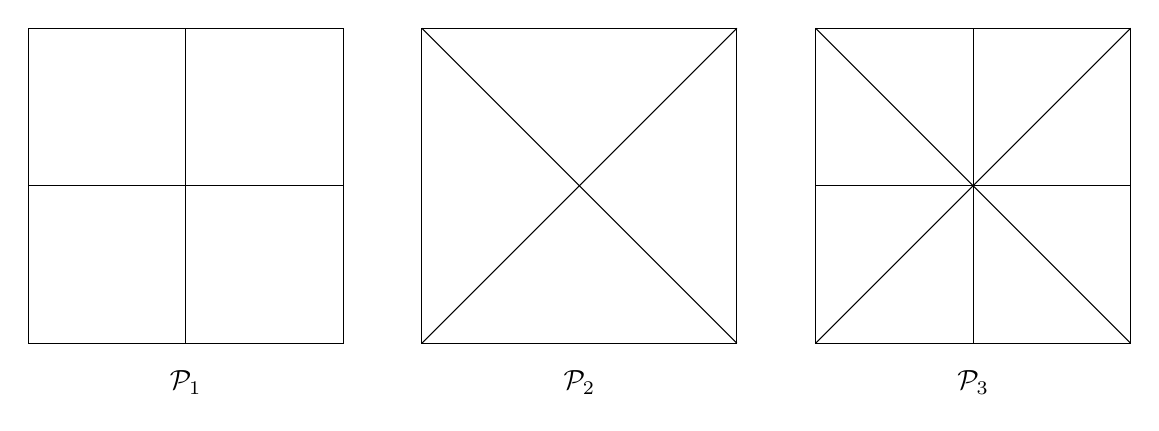
\begin{tikzpicture}
    % Outer square
    \draw (0,0) rectangle (4,4);

    % Vertical and horizontal dividing lines
    \draw (2,0) -- (2,4);
    \draw (0,2) -- (4,2);

    % Outer square
    \draw (5,0) rectangle (9,4);

    % Diagonals
    \draw (5,0) -- (9,4); % Diagonal from bottom-left to top-right
    \draw (5,4) -- (9,0); % Diagonal from top-left to bottom-right
    
    % Outer square
    \draw (10,0) rectangle (14,4);

    % Diagonals
    \draw (10,0) -- (14,4); % Diagonal from bottom-left to top-right
    \draw (10,4) -- (14,0); % Diagonal from top-left to bottom-right
    \draw (10,2) -- (14,2);
    \draw (12,0) -- (12,4);
    
    \node at (2, -0.5) {$\P_1$}; % Label beneath the square
    \node at (7, -0.5) {$\P_2$}; % Label beneath the square
    \node at (12, -0.5) {$\P_3$}; % Label beneath the square
  \end{tikzpicture}
  \caption{Example of 2 partions of the square $\P_1$ and $\P_2$ with common upper bound $\P_3$.}
\end{figure}

\begin{rem}\label{rem:partfinsze}
  If $X$ is an infinite set then $\Pi(X)$ is also infinite.
\end{rem}

\begin{proof}
  Define $\P \subseteq \Pi(X)$ as follows
  \begin{equation*}
    \P := \Big\{ \{ \{x\}, \: X\setminus\{x\}\}\colon \: \forall x \in X \Big\}.
  \end{equation*}
  It is now clear that $\left| \P \right| = \left| X \right|$ and since $\P \subseteq \Pi(X)$ it follows that 
  \begin{equation*}
    \left| X \right| \leq \left| \Pi(X) \right|.
  \end{equation*}
\end{proof}

\clearpage

\topskip0pt
\vspace*{\fill}
\noindent
\textbf{Eidesstattliche Versicherung}

\noindent
Hiermit versichere ich, dass ich die vorliegende Arbeit selbstständig und ohne unerlaubte Hilfe angefertigt und andere als die in der Arbeit angegebenen Hilfsmittel nicht benutzt habe. Alle Stellen, die wörtlich oder sinngemäß aus anderen Schriften entnommen sind, habe ich als solche kenntlich gemacht.
\vspace*{50px}

\noindent
Freiberg, 12. Februar, 2025  
\vspace*{\fill}

\clearpage
\printbibliography

\end{document}
